\documentclass[12pt, twoside]{article}
\usepackage[letterpaper, margin=1in, headsep=0.2in]{geometry}
\setlength{\headheight}{0.6in}
%\usepackage[english]{babel}
\usepackage[utf8]{inputenc}
\usepackage{microtype}
\usepackage{amsmath}
\usepackage{amssymb}
%\usepackage{amsfonts}
\usepackage{siunitx} %units in math. eg 20\milli\meter
\usepackage{yhmath} % for arcs, overparenth command
\usepackage{tikz} %graphics
\usetikzlibrary{quotes, angles}
\usepackage{graphicx} %consider setting \graphicspath{{images/}}
\usepackage{parskip} %no paragraph indent
\usepackage{enumitem}
\usepackage{multicol}
\usepackage{venndiagram}

\usepackage{fancyhdr}
\pagestyle{fancy}
\fancyhf{}
\renewcommand{\headrulewidth}{0pt} % disable the underline of the header
\raggedbottom
\hfuzz=2mm %suppresses overfull box warnings

\usepackage{hyperref}

\fancyhead[LE]{\thepage}
\fancyhead[RO]{\thepage \\ Name: \hspace{4cm} \,\\}
\fancyhead[LO]{BECA / Dr. Huson / Geometry\\*  Unit 2: Angles\\* 12 October 2022}

\begin{document}

\subsubsection*{2.5 Homework: Angle terminology and angle addition}
\begin{enumerate}
\item Use standard notation to represent an angle, the angle symbol followed by three letters, $\angle ABC$. \vspace{0.25cm}
  \begin{enumerate}
    \item Name a right angle: \rule{4cm}{0.15mm} \bigskip
    \item Name the angle vertical to $\angle LXM$: \rule{4cm}{0.15mm}  \bigskip 
    \item Name the ray opposite to $\overrightarrow{XJ}$: \rule{4cm}{0.15mm} \bigskip
    \item What is the measure of $\angle KXM$?  \rule{4cm}{0.15mm} \bigskip
    \item Are $\angle JXL$ and $\angle LXM$ complementary, supplementary, or neither?
  \end{enumerate}
  \begin{center}
  \begin{tikzpicture}[scale=0.7, rotate=30]
    \draw[<->, thick] (-110:2)--(0,0)--(70:3);
    \draw[<->, thick] (-4,0)--(3,0);
    \draw[->, thick] (0,0)--(0,3);
    \draw (0,0)++(-0.3,0)--++(0,0.3)--+(0.3,0);
    \draw[fill] (70:2) circle [radius=0.05] node[right]{$L$};
    \draw[fill] (-3,0) circle [radius=0.05] node[above left]{$J$}; 
    \draw[fill] (0,0) circle [radius=0.05] node[below right]{$X$};
    \draw[fill] (0,2) circle [radius=0.05] node[left]{$K$};
    \draw[fill] (2,0) circle [radius=0.05] node[below right]{$M$};
    \draw[fill] (-110:1.5) circle [radius=0.05] node[right]{$N$};
  \end{tikzpicture}
  \end{center}

\item The size of an angle is its ``measure,'' which can be from $0^\circ$ to $360^\circ$
\begin{enumerate}
  \item What is the degree measure of the angle, m$\angle PQR$?  \par \medskip
  \begin{tikzpicture}[scale=0.7, rotate=-20]
    \draw[<->, thick] (4,0)--(0,0)--(0,3);
    \draw (0,0)++(0.3,0)--++(0,0.3)--+(-0.3,0);
    \draw[fill] (0,0) circle [radius=0.05] node[below]{$Q$};
    \draw[fill] (0,2) circle [radius=0.05] node[right]{$P$};
    \draw[fill] (3,0) circle [radius=0.05] node[above]{$R$};
  \end{tikzpicture}
  \item What is the degree measure made by these two opposite rays, $\overrightarrow{BA}$ and $\overrightarrow{BC}$?
  \begin{flushright}
    \begin{tikzpicture}[scale=.8, rotate=50]
      \draw  [<->, thick] (0,2)--(4,0);
      \draw[fill] (1,1.5) circle [radius=0.05] node[below]{$A$};
      \draw[fill] (2,1) circle [radius=0.05] node[below]{$B$};
      \draw[fill] (3,0.5) circle [radius=0.05] node[below]{$C$};
    \end{tikzpicture}
  \end{flushright}
    \item The given angle $\angle UVW$ is which of the following: acute, obtuse, or right?
    \begin{center}
      \begin{tikzpicture}[scale=.8]
        \draw  [<->, thick] (-3,0)--(0,0)--(45:3);
        \draw[fill] (-2,0) circle [radius=0.05] node[below]{$U$};
        \draw[fill] (0,0) circle [radius=0.05] node[below]{$V$};
        \draw[fill] (45:2) circle [radius=0.05] node[above left]{$W$};
      \end{tikzpicture}
    \end{center}
  \end{enumerate}

\item As shown below, two lines intersect making four angles: $\angle 1$, $\angle 2$, $\angle 3$, and $\angle 4$.
  \begin{multicols}{2}
    Given m$\angle 2 = 120^\circ$.  
    \begin{enumerate}
      \item Find m$\angle 3$ \vspace{1cm}
      \item Find m$\angle 4$ \vspace{2cm}
    \end{enumerate} \vspace{2cm}
    \begin{tikzpicture}[scale=0.7, rotate=20]
    \draw[<->, thick] (0,-1.5)--(10,1.5);
    \draw[<->, thick] (2,3.5)--(7,-3.5);
    \node at (3,.4){1};
    \node at (6,-.6){3};
    \node at (5,1){2};
    \node at (4,-1){4};
  \end{tikzpicture}
  \end{multicols}

\subsubsection*{Angle addition situations}
\item Apply the Angle Addition postulate. Write and equation to support your work.
  \begin{multicols}{2}
    Given m$\angle CBD = 30^\circ$, m$\angle ABC = 90^\circ$.  \par \bigskip
    Find $m \angle ABD$.  \par
    \begin{tikzpicture}[scale=1.4]
      \draw[<->, thick]
        (0:3) coordinate (a) node[below left] {$C$}
        -- (0,0) coordinate (b) node[below left] {$B$}
        -- (30:3) coordinate (c) node[below right] {$D$}
        pic["$30^\circ$", <->, draw=black, angle eccentricity=1.5, angle radius=1cm]
        {angle=a--b--c};
        \draw[<-, thick]
        (90:2) coordinate (d) node[right] {$A$}
        -- (0,0) coordinate (e)
        pic["$?$", <->, draw=black, angle eccentricity=1.25, angle radius=1cm]
        {angle=c--e--d};
      \draw (0,0)++(0.3,0)--++(0,0.3)--+(-0.3,0);
    \end{tikzpicture}
  \end{multicols}

\item Given m$\angle ABD = x+20$, m$\angle DBC = 4x$, and $m \angle ABC = 120^\circ$, as shown.  \par \medskip
  Write an equation and solve for $x$.
  \begin{flushright}
      \begin{tikzpicture}[scale=1.8]
        \draw[<->, thick]
          (-20:1.5) coordinate (a) node[below left] {$C$}
          -- (0,0) coordinate (b) node[below left] {$B$}
          -- (65:2) coordinate (c) node[below right] {$D$}
          pic["\hspace{1cm}$4x$", <->, draw=black, angle eccentricity=1, angle radius=1.5cm]
          {angle=a--b--c};
          \draw[<-, thick]
          (100:1.75) coordinate (d) node[below left] {$A$}
          -- (0,0) coordinate (e)
          pic["$x+20$", <->, draw=black, angle eccentricity=1.25, angle radius=2cm]
          {angle=c--e--d};
      \end{tikzpicture}
    \end{flushright}
    Show your check for full credit.

\newpage
\item Given $\overrightarrow{BD} \perp \overleftrightarrow{ABC}$, m$\angle DBE = 2x$, and m$\angle EBC = x - 15^\circ$, as shown below.  \par \bigskip 
  Write an equation and solve for $x$.
    \begin{flushright}
      \begin{tikzpicture}[scale=1.3]
        \draw[<->, thick]
          (0:5) coordinate (a) node[below left] {$C$}
          -- (0,0) coordinate (b) node[below] {$B$}
          -- (35:5) coordinate (c) node[below right] {$E$}
          pic["$x-15$", <->, draw=black, angle eccentricity=2, angle radius=1cm]
          {angle=a--b--c};
          \draw[<-, thick]
          (90:3) coordinate (d) node[right] {$D$}
          -- (0,0) coordinate (e)
          pic["\hspace{0.3cm}$2x$", <->, draw=black, angle eccentricity=1.6, angle radius=1cm]
          {angle=c--e--d};
          \draw[->, thick] (0,0)--(-180:2) node[below right]{$A$};
          \draw (0,0)++(-0.3,0)--++(0,0.3)--+(0.3,0);
      \end{tikzpicture}
    \end{flushright}

\item A linear pair is formed by two angles, m$\angle RUT = 2x+5$ and m$\angle SUT = x + 55^\circ$.  \par \bigskip 
  Write an equation, then solve for $x$. \vspace{0.5cm}
    \begin{flushright}
    \begin{tikzpicture}[scale=1]
      \draw[<->, thick]
        (0:5) coordinate (a) node[below left] {$S$}
        -- (0,0) coordinate (b) node[below] {$U$}
        -- (95:3) coordinate (c) node[above right] {$T$}
        pic["$x+55^\circ$", <->, draw=black, angle eccentricity=1.5, angle radius=1.5cm]
        {angle=a--b--c};
        \draw[<-, thick]
        (180:4) coordinate (d) node[below] {$R$}
        -- (0,0) coordinate (e)
        pic["$2x+5$", <->, draw=black, angle eccentricity=1.5, angle radius=1.5cm]
        {angle=c--e--d};
    \end{tikzpicture}
    \end{flushright}
      
\item In the diagram shown, $\overrightarrow{BD} \perp \overleftrightarrow{ABC}$ and angle measures are given.  \par \bigskip 
  Find $x$. Show the check for full credit.\vspace{0.5cm}
    \begin{multicols}{2}
      m$\angle DBE = 4x+4^\circ$  \par \medskip
      m$\angle EBC = 9x-5^\circ$  \par \medskip
      \begin{tikzpicture}[scale=1]
        \draw[<->, thick]
          (0:5) coordinate (a) node[below left] {$C$}
          -- (0,0) coordinate (b) node[below] {$B$}
          -- (50:5) coordinate (c) node[below right] {$E$}
          pic["$9x-5$", <->, draw=black, angle eccentricity=1.5, angle radius=1.5cm]
          {angle=a--b--c};
          \draw[<-, thick]
          (90:4) coordinate (d) node[right] {$D$}
          -- (0,0) coordinate (e)
          pic["$4x+4$", <->, draw=black, angle eccentricity=1.5, angle radius=1.5cm]
          {angle=c--e--d};
          \draw[->, thick] (0,0)--(-180:2) node[below right]{$A$};
          \draw (0,0)++(-0.3,0)--++(0,0.3)--+(0.3,0);
      \end{tikzpicture}
    \end{multicols}

\newpage
\item Given $\overleftrightarrow{ABC}$, right angle $\angle DBE$, m$\angle ABE = 3x+6$, and m$\angle DBC = 2x-1$.  \par \bigskip 
  Find m$\angle ABE$. \vspace{0.5cm}
    \begin{flushright}
      \begin{tikzpicture}[scale=1, rotate=30]
        \draw[<->, thick]
          (-30:5) coordinate (a) node[below left] {$C$}
          -- (0,0) coordinate (b) node[below] {$B$}
          -- (3,0) coordinate (c) node[below right] {$D$}
          pic["$2x-1$", <->, draw=black, angle eccentricity=1.5, angle radius=1.5cm]
          {angle=a--b--c};
          \draw[<->, thick]
          (150:4) coordinate (d) node[below] {$A$}
          -- (0,0) -- (0, 3) coordinate (e) node[right] {$E$}
          pic["$3x+6$", <->, draw=black, angle eccentricity=1.5, angle radius=1.5cm]
          {angle=e--b--d};
          \draw (0,0)++(0.4,0)--++(0,0.4)--+(-0.4,0);
      \end{tikzpicture}
    \end{flushright}

\item Ray $\overrightarrow{BF}$ is the angle bisector of $\angle ABC$. Given that the angle measures are m$\angle ABF = 7x-14$ and m$\angle CBF = 5x+10$.  \par \bigskip 
  Find $x$. \vspace{0.5cm}
    \begin{flushright}
      \begin{tikzpicture}[scale=1]
        \draw[<->, thick]
          (0:5) coordinate (a) node[below left]{$C$}
          -- (0,0) coordinate (b) node[below]{$B$}
          -- (70:3) coordinate (c) node[above right]{$F$}
          pic["$5x+10$", <->, draw=black, angle eccentricity=1.75, angle radius=1.5cm]
          {angle=a--b--c};
          \draw[<-, thick]
          (140:4) coordinate (d) node[below left]{$A$}
          -- (0,0) coordinate (e)
          pic["$7x-14$", <->, draw=black, angle eccentricity=1.25, angle radius=1.5cm]
          {angle=c--e--d};
      \end{tikzpicture}
    \end{flushright} \vfill

\item Find the height of the $\triangle RST$, having an area of $A=117$ and base $RS=9$.
\begin{multicols}{2}
  Start by substituting values in the area formula: \\[0.5cm]
  $\displaystyle A = \frac{1}{2} bh = 117$ \vspace{2cm}
    \begin{flushright}
    \begin{tikzpicture}[scale=.635]
      %\draw[help lines] (-1,-1) grid (9,6);
      \draw[thick, ->] (-1.2,0) -- (9.4,0) node [below right] {$x$};
      \draw[thick, ->] (0,-1.2)--(0,8.4) node [left] {$y$};
      \draw[<->, thick] (1.5,1)--(1.5,7);
      \draw[thick] (2,1)--(6,1)--(4,7)--cycle;
      \draw[dashed] (6,1)--(8,7)--(4,7);
      \draw[fill] (2,1) circle [radius=0.05] node[below] {$R$};
      \draw[fill] (6,1) circle [radius=0.05] node[below] {$S$};
      \draw[fill] (4,7) circle [radius=0.05] node[above right] {$T$};
      \node at (4,1)[below]{$9$};
      \node at (1.5,4)[left]{$h$};
    \end{tikzpicture}
    \end{flushright}
\end{multicols}

\end{enumerate}
\end{document}